\documentclass[openany]{book}

\input{../../../latex_preambule_style/preambule}
\input{../../../latex_preambule_style/styleCoursCycle4}
\input{../../../latex_preambule_style/styleExercices}
\input{../../../latex_preambule_style/styleExercicesAideCompetences}
%\input{../../latex_preambule_style/styleCahier}
\input{../../../latex_preambule_style/bas_de_page_cycle4}
\input{../../../latex_preambule_style/algobox}


%%%%%%%%%%%%%%%  Affichage ou impression  %%%%%%%%%%%%%%%%%%
\newcommand{\impress}[2]{
\ifthenelse{\equal{#1}{1}}  %   1 imprime / affiche sur livre  -----    0 affiche sur cahier 
{%condition vraieé
#2
}% fin condition vraie
{%condition fausse
}% fin condition fausse
} % fin de la procédure
%%%%%%%%%%%%%%%  Affichage ou impression  %%%%%%%%%%%%%%%%%%
 \usepackage{geometry}
 \geometry{top=2.5cm, bottom=0cm, left=2cm , right=2cm}
%%%%%%%%%%%%%%%%%%%%%%%%%%%%%%%%%%%%%%%%%%%%%%%%

\begin{document}

\begin{seance}[Equations et ordre]

\begin{description}
\item[$\square$] Résoudre de façon exacte ou approchée des problèmes du premier degré
\end{description}
\end{seance}

\Exe


Pour quelle valeur de $x$ l'égalité $\frac{2}{x-3}=0,5$ est elle vraie ? 

\hfill{{\scriptsize Source : http://laroche.lycee.free.fr/telecharger/2nde/problemes\_ouverts\_6a2.pdf}}

\Exe


\begin{description}
\item[Problème 1 :] 4 boissons à 2,5 € et 3 menus identiques coûtent 52,00 €. Quel est le prix d'un menu ?
\item[Problème 2 :] Un rectangle de largeur 3 cm a pour périmètre 24 cm. Quel est la longueur d'un rectangle ?
\end{description}



\Exe


On donne l'algorithme suivant.

\begin{algobox}
\Variables
\Ligne $x$ EST\_DU\_TYPE NOMBRE
\DebutAlgo
\Ligne Multiplie $x$ par 2
\Ligne Ajoute 5
\FinAlgo
\end{algobox}



\begin{enumerate}
\item Quelle est l'expression renvoyée en fonction de $x$ ?
\item Quelle valeur obtient-on pour $x= -5$ ?
\item Pour quelle valeur de $x$ obtient-on 75 ?
\end{enumerate}




\Exe


\begin{center}
 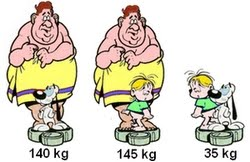
\includegraphics[scale=0.5]{EO-11.jpg}
 \end{center} 

En utilisant les informations données par ces trois dessins, détermine combien pèsent le gros Dédé, le petit Francis et
le chien Boudin.

\Exe

Pour travailler la technique en autonomie : https://ggbm.at/rKKK6wQW


\begin{seance}[Equations et ordre]

\begin{description}
\item[$\square$] Résoudre une inéquation du premier degré
\item[$\square$] Faire le lien entre forme algébrique et représentation graphique
\end{description}
\end{seance}

\Exe


Un vidéo club propose 2 sortes de location de DVD.

\begin{center}
\begin{tabular}{|c|c|}
 \hline 
 Option 1 &  Option 2 \\ 
  \hline
 abonnement annuel de 20 \euro{} &  sans abonnement \\
 + 4 \euro par DVD loué & 6,5 \euro par DVD loué \\ 
 \hline 
 \end{tabular}  
\end{center}

\begin{enumerate}
\item Calculer le cout annuel pour 6 DVD loués avec chaque option.
\item Estelle a payé 91 \euro{} pour 14 DVD loués. 
\begin{enumerate}
\item Quelle formule a-t-elle choisi ? 
\item Que penses-tu de son choix ?
\end{enumerate}
\item Quelle est l'option la plus rentable selon le nombre de DVD ?
\end{enumerate}

\begin{DefT}{Inéquation}
On appelle \textbf{inéquation}\index{Inéquation} une proposition mathématique qui compare deux expressions dont au moins une contient une inconnue. 

\textbf{Résoudre une inéquation} \index{Inéquation!Résoudre}, c'est déterminer toutes les valeurs de l'inconnue qui vérifient la comparaison entre les deux membres.
\end{DefT}

\begin{Reg}
\begin{enumerate}
\item Lorsqu'on ajoute (ou soustrait ) un \textbf{même} nombre à \textit{chaque membre} de l'inéquation, l'ordre ne change pas.
\item Lorsqu'on multiplie (ou divise ) un \textbf{même} nombre \textbf{positif non nul} à \textit{chaque membre} de l'inéquation, l'ordre ne change pas.
\item \rotatebox{90}{{\color{red}$\blacktriangleright$}} Lorsqu'on multiplie (ou divise ) un \textbf{même} nombre \textbf{négatif non nul} à \textit{chaque membre} de l'inéquation, l'ordre change.
\end{enumerate}
\end{Reg}


\begin{Mt}   
On souhaite résoudre l'inéquation $x + 7 < 5$
\begin{description}
\item[1a. Isoler $x$.] En soustrayant 7 à chaque membre, on obtient : $x + 7 - 7 < 5 - 7$. L'ordre ne change pas car on opère une soustraction.
\item[1b. Simplifier.]  $x +0 < - 2$ 
\item[1c. Réduire.]  $x < - 2$  
\item[2. Conclure.] La solution est composée de tous les nombres strictement inférieurs  à $-2$.
\item[3. Représentation] On représente l'ensemble solution sur la droite graduée, ici en rouge :
 
\begin{tikzpicture}[line cap=round,line join=round,>=triangle 45,x=0.5cm,y=1.0cm]
\draw[->,color=black] (-10.193119401716665,0.) -- (10.5522947678536005,0.);
\foreach \x in {-10.,-8.,-6.,-4.,-2.,2.,4.,6.,8.,10.}
\draw[shift={(\x,0)},color=black] (0pt,2pt) -- (0pt,-2pt) node[below] {\footnotesize $\x$};
\draw[color=black] (0pt,-10pt) node[right] {\footnotesize $0$};
\clip(-10.193119401716665,-0.5) rectangle (10.5522947678536005,0.5);
\draw [line width=3.4pt,color=red] (-2.,0.)-- (-12.,0.);
\end{tikzpicture}
\end{description}
\end{Mt} 

\begin{Mt}   
On souhaite résoudre l'inéquation $-2x - 5 \geq 11 $
\begin{description}
\item[1a. Isoler $x$.] En ajoutant 5 à chaque membre, on obtient :  $-2x - 5 +5 \geq 11 +5 $. L'ordre ne change pas car on opère une addition.
\item[1b. Simplifier.]  $-2x  \geq 16 $.
\item[2a. Diviser.]  $\frac{-2}{-2}x  \leq \frac{16}{-2}$. On divise chaque membre par $-2 <0$. Donc {\color{red}l'ordre change}.  
\item[2b. Simplifier.]  $x  \leq -8$  
\item[2. Conclure.] La solution est composée de tous les nombres inférieurs ou égaux à $-8$.
\item[3. Représentation]
On représente l'ensemble solution sur la droite graduée, ici en rouge : 

\begin{tikzpicture}[line cap=round,line join=round,>=triangle 45,x=0.5cm,y=1.0cm]
\draw[->,color=black] (-20.193119401716665,0.) -- (2.5522947678536005,0.);
\foreach \x in {-20.,-18.,-16.,-14.,-12.,-10.,-8.,-6.,-4.,-2.,2.}
\draw[shift={(\x,0)},color=black] (0pt,2pt) -- (0pt,-2pt) node[below] {\footnotesize $\x$};
\draw[color=black] (0pt,-10pt) node[right] {\footnotesize $0$};
\clip(-20.193119401716665,-1.262783989122121) rectangle (2.5522947678536005,1.1022719129769702);
\draw [line width=3.4pt,color=red] (-7.929866576017677,0.)-- (-22.96695039800572,0.);
\end{tikzpicture}
\end{description}
\end{Mt} 

\Exe

Pour travailler en autonomie la technique.

https://ggbm.at/mJKc4mVJ


\Exe


Le périmètre d’un rectangle est inférieur ou égal à 37 cm. Sachant que sa largeur est égale à 5,3 cm, déterminer les valeurs possibles pour la longueur de ce rectangle. (La longueur doit être supérieure à la largeur) 



\begin{seance}[Equations et ordre]

\begin{description}
\item[$\square$] Résoudre une équation produit
\item[$\square$] Faire le lien entre forme algébrique et représentation graphique
\end{description}
\end{seance}

\begin{DefT}{Équation produit nul}
On appelle \textbf{équation produit nul}\index{Équation produit nul} une équation dont l'un des membres est un produit de facteurs et l'autre est 0. 
\end{DefT}


\begin{Mt}[. Résolution d'une équation produit nul]\index{Équation produit nul!Résolution}

\begin{tabular}{ccc}
\multicolumn{3}{c}{$(2x-1)(x+3)=0$} \\ 
\multicolumn{3}{c}{un produit est nul lorsqu'au moins un de ses facteurs est nul. }\\  
$2x-1=0$ & ou & $x+3=0$ \\  
$2x=1$ & ou & $x=-3$ \\ 
$x=\frac{1}{2}$ &  &  \\ 
\multicolumn{3}{c}{$S=\left\lbrace \frac{1}{2}; -3 \right\rbrace $}\\  
\end{tabular} 
\end{Mt}

\Exe


Résous les équations suivantes.

\begin{description}
\begin{minipage}{0.3\linewidth}
\item[a. ] $(x-1)(x+3)=0$
\item[b. ] $(x+2)(2x-1)=0$
\item[c. ] $(3-2x)(-x+5)=0$
\end{minipage}
\begin{minipage}{0.3\linewidth}
\item[d. ] $2x(x-1)(5-2x)=0$
\item[e. ] $(5x-1)(7-x)=0$
\item[f. ] $(2-3x)(x+1)=0$
\end{minipage}
\begin{minipage}{0.3\linewidth}
\item[g. ] $(x-1)^2-4=0$
\item[h. ] $16-(x+2)^2=0$
\item[i. ] $9-(-x+5)^2=0$
\end{minipage}
\end{description}

\Exe

Soit $x$ un nombre.
\begin{enumerate}
\item Factoriser $x^2-4+x-2$
\item En déduire un ensemble solution de $x^2-4+x-2=0$
\item Vérifier que pour tout réel nombre $x$, $x^2+x-6=0$
\item En déduire un ensemble solution de $x^2+x-6=0$
\end{enumerate}

\Exe

\begin{enumerate}
\item Factoriser astucieusement $9-x^2+x+3$
\item En déduire les solutions de l'équation $-x^2+x+12=0$
\end{enumerate}

\Exe

\begin{enumerate}
\item Factoriser astucieusement $4x^2-25+2x-5$.
\item En déduire les solutions de l'équation $4x^2+2x-30=0$.
\end{enumerate}




\end{document}